\documentclass[a4paper, 11pt]{article}
\usepackage[serbian]{babel}
\usepackage{hyperref}
\usepackage{graphicx}
\usepackage{listings}
\usepackage{xparse}
\usepackage{multicol}

\usepackage{xcolor}
 
\definecolor{codegreen}{rgb}{0,0.6,0}
\definecolor{codegray}{rgb}{0.5,0.5,0.5}
\definecolor{codepurple}{rgb}{0.58,0,0.82}
\definecolor{backcolour}{rgb}{0.95,0.95,0.92}
 
\lstdefinestyle{mystyle}{
    backgroundcolor=\color{backcolour},   
    commentstyle=\color{codegreen},
    keywordstyle=\color{magenta},
    numberstyle=\tiny\color{codegray},
    stringstyle=\color{codepurple},
    basicstyle=\ttfamily\footnotesize,
    breakatwhitespace=false,         
    breaklines=true,                 
    captionpos=b,                    
    keepspaces=true,                 
    numbers=left,                    
    numbersep=5pt,                  
    showspaces=false,                
    showstringspaces=false,
    showtabs=false,                  
    tabsize=2
}
 
\lstset{style=mystyle}



\title{\large Seminarski rad iz predmeta Istra\v zivanje podataka 1
		\\ Podaci: FIFA19 }
\author{Nikola Jankovi\'c 
		\\ e-mail: \href{mailto:nikola_jankovic@tuta.io}{nikola\_jankovic@tuta.io}
		\\ \\ \small{Matemati\v cki fakultet, Univerzitet u Beogradu}
} 




\begin{document}


\begin{titlepage}
\maketitle
\thispagestyle{empty}

\begin{abstract}
Tema ovog seminarskog rada je detaljnija analiza, sa klasterovanjem,
skupa podataka dobijenog iz poslednje verzije
igrice FIFA19 (u toku pisanja rada) preuzetog sa adrese: \url{https://www.kaggle.com/karangadiya/fifa19}.
U radu \'{c}e biti prikazani neki od algoritama za klasterovanje i rezultati dobijeni primenom na ovaj skup.
Uz poku\v{s}aj da budu dobijeni klasteri što pribli\v{z}niji nekim podelama koje postoje u fudbalu. 
\end{abstract}

\end{titlepage}

\tableofcontents

\section{Uvod}



Klaster analiza je grupisanje objekata koje se oslanja samo na informacije koje se nalaze u podacima
koji opisuju te objekte i veze me\dj u njima. Cilj klaster analize je da objekti u grupi budu sli\v{c}ni(povezani) me\dj{}usobno i druga\v{c}iji od objekata u drugim grupama.
\v{S}to je ve\'{c}a sli\v{c}nost u grupi i razli\v{c}itost me\dj{}u grupama klaster analiza je 
izrazitija. \\
U ovom seminarskom radu bi\'{c}e prikazani rezultati klaster analize pomo\'{c}u algoritama
koji su vi\dj{}eni na kursu Istra\v{z}ivanje podataka 1:
\begin{itemize}
\item K-means
\item DBSCAN
\item Self Organizing Maps (\emph{Kohonen})
\item Hijerahijsko klasterovanje
\end{itemize} 
kao i dva dodatna algoritma:
\begin{itemize}
\item Mean-Shift
\item BIRCH
\end{itemize}


Svi algoritmi su primenjeni uz pomo\'{c} biblioteka jezika Python uz
kori\v{s}enje softvera IBM Spss Modeler zbog lo\v{s}e dokumentacije
vezane za SOM\footnote{Self Organizing Maps} u modulu \emph{minisom\footnote{\url{https://github.com/JustGlowing/minisom}}}.


\subsection{Skup podataka kori\v{s}\'{c}en u radu}
Skup podataka sastoji se od $\approx 18000$ igra\v{c}a(\emph{slogova}) i 89 ocena(\emph{atributa}).
Blagi uvid u tabelu je mogu\'{c} na slici 1. 
\begin{figure}[h]
\graphicspath{{../}}
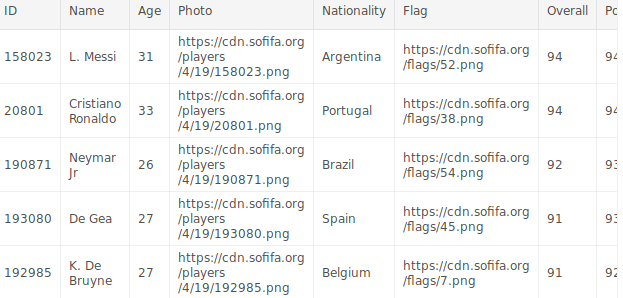
\includegraphics[scale=0.45]{head.png}
\caption{data.csv}
\label{data}
\end{figure}

Podaci iz skupa se koriste kao parametri koje koristi kompanija \emph{EA Sports}
pri kreiranju simulacije fudbalera iz realnog sveta kako bi napravili
distinkciju me\dj{}u njima.
\\
Nazivi kolona uglavnom nedvosmisleno ukazuju na njihovo zna\v{c}enje, ali \'{c}e 
ipak biti data obja\v{s}njenja za neke od atributa, koje korisnik smatra da nisu
poznati ve\'{c}ini.
\begin{itemize}

\item \emph{Value} - Predstavlja procenjenu trenutnu vrednost igra\v{c}a u dolarima, potrebno je praviti
razliku u odnosu na atribut \emph{Release Clause}

\item \emph{International Reputation} - Broj izme\dj{}u 0 i 1 koji govori koliko je uspeha imao u igrama za 
reprezentaciju svoje zemlje.

\item \emph{Loaned from} - Pojedini igra\v{c}i mogu biti posu\dj{}eni timu X od strane tima Y. Do kraja
posudbe tim X je u obavezi da pla\'{c}a igra\v{c}a u istom iznosu kao \v{s}to je to radio
tim Y. Na kraju posudbe tim X ima prednost (u nekim slu\v{c}ajevima i pravo) da otkupi u potpunosti
prava na igra\v{c}a od tima Y.

\item \emph{LS, ST, RS, ..., RB} - Atributi koji predstavljaju koliko je projektovana Overall ocena
igra\v{c}a u slu\v{c}aju da ga osoba koja igra igricu postavi na poziciju sa tim nazivom kolone.

\item \emph{Release Clause} - Procenjena cena koju je potrebno da tim Y plati timu X kako bi otkupio prava
na igra\v{c}a, \v{c}esto je vrednost ovog atributa ve\'{c}a u odnosu na atribut \emph{Value}, pogotovo kod
mla\dj{}ih igra\v{c}a.
\end{itemize}

\section{Analiza podataka}

U ovom delu bi\'{c}e izlo\v{z}ene neke zanimljive statistike iz skupa
i prikazano kako je izvr\v{s}eno pretprocesiranje podataka

\subsection{Statistike}
Na slici 2. mo\v{z}emo videti dijagaram zajedni\v{c}ke gustine raspodele
za ocene \emph{Overall} i \emph{Age}

\begin{figure}[h]
\centering
\graphicspath{{../}}
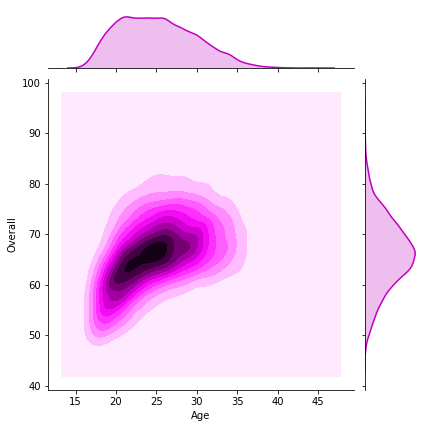
\includegraphics[scale=0.45]{stat1.png}
\caption{Dijagram odnosa Age $\sim$ Overall}

\end{figure}

Vidimo da je raspodela za \emph{Overall} normalna, dok
\emph{Age} podse\'{c}a na neku $\tilde{\chi}^2$ raspodelu.
Kao i da najve\'{c}i broj fudablera ima izme\dj{}u 23 i 27 godina
sa \emph{Overall} od 60 do 70 (potpuno o\v{c}ekivano).

\pagebreak

Druga zanimljiva statistika nam pokazuje raspodelu za atribut
\emph{Release Clause} i lako se uo\v{c}ava da najve\'{c}a koli\v{c}ina
novca figurira  u malom procentu igra\v{c}a. Dok je kod igra\v{c}a
koji nisu vrhunske klase to zna\v{c}ajno manje.


\begin{figure}[h]
\centering
\graphicspath{{../}}
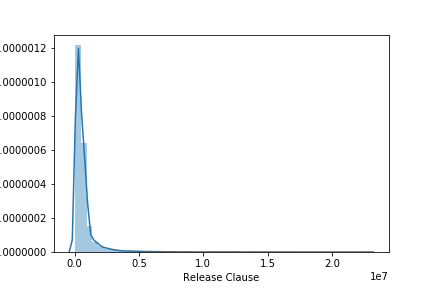
\includegraphics[scale=0.45]{stat2.png}
\caption{Raspodela izlazne klauze}

\end{figure}




I tre\'{c}i dijagram nam pokazuje koliko igra\v{c}a nam dolazi 
iz koje dr\v{z}ave (razmatrane samo dr\v{z}ave koje imaju vi\v{s}e od 500 predstavnika)


\begin{figure}[h]
\centering
\graphicspath{{../}}
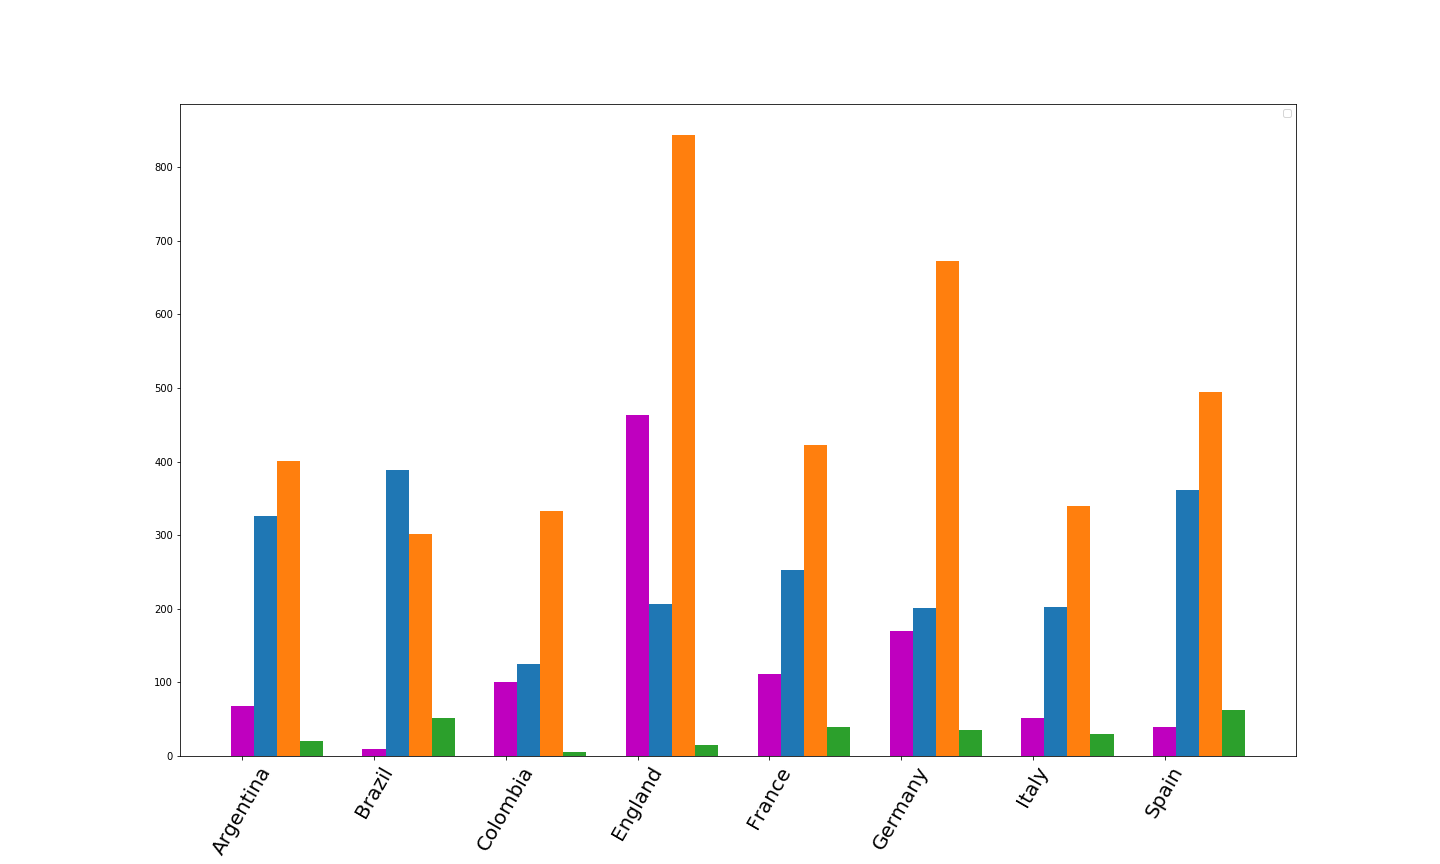
\includegraphics[scale=0.285]{stat3.png}
\caption{}

\end{figure}

Primetno je da je broj igra\v{c}a iz Engleske najve\'{c}i kao
i da dominiraju u broju igra\v{c}a sa ocenom manjom od 60.
Razlog ovome je to \v{s}to u igrici postoje timovi iz \v{c}ak
4 engleska liga\v{s}ka takmi\v{c}enja u kojima ve\'{c}inu \v{c}ine
igra\v{c}i iz Engleske, a kako su timovi iz 3. i 4. ranga polu-profesionalni,
ocene za igra\v{c}e su o\v{c}ekivano niske.
\pagebreak

\subsection{Pretprocesiranje}
U po\v{c}etku skup se sastoji od 89 atributa, od kojih $\approx 55 $ su numeri\v{c}ki
dok su ostali \v{s}to ordinalni \v{s}to nominalni.
 
Prvi korak je bio eliminacija jednog broja kvalitativnih atributa koji nisu mogli nikako
biti kori\v{s}\'{c}eni u ovoj klaster analizi. Kao na primer:
\emph{ID, Name, Photo, Club, Club Logo, Flag, Jersey Number, Loaned From, Work Rate, Real Face, 
Joined, Body Type}. \\

\begin{itemize}



\item Atribut \emph{Body Type} je ordinalni atrbiut u vidu stringa sa nekoliko vrednosti: C.Ronaldo, L.Messi, X.Shaqiri kao i vrednstima visok, nizak, zdepast. Pritom atributi \emph{Height i Weight} obja\v{s}njavaju
sli\v{c}nu stvar na mnogo egzaktniji na\v{c}in. \\
\item Tako\dj{}e atribut \emph{Club} bi se mogao mapirati u numeri\v{c}ke vrednosti koje predstavljaju
snagu kluba u svetskim okvirima. Na \v{z}alost takvu bazu vodi samo evropska fudbalska asocijacija za 
klubove iz Evrope, dok u skupu podataka ovog seminarskog rada se nalaze podaci o
igra\v{c}ima koji igraju \v{s}irom sveta.

\end{itemize}


Slede\'{c}i korak u ovom delu je bio izbacivanje atributa \emph{LS, ST, RS, ..., RB} jer su oni zapravo
nastali iz ostalih numeri\v{c}kih atributa koji predstavljaju kvalitet igra\v{c}eve igre. Pa su izba\v{c}eni
kako bi ubrzali rad algoritama.

Neki od numeri\v{c}kih atributa su dati u vidu stringa, pa je njih bilo neophodno parsirati i pretvoriti u 
Python numeri\v{c}ki tip. To su uglavnom atributi koji predstavljaju nov\v{c}ane vrednosti
kao na primer \emph{Wage, Value, Release Clause}.
U nastavku je fragment koda kojim je re\v{s}en ovaj problem.

\begin{lstlisting}[language=Python] 
df['Release Clause'] = df['Release Clause'].replace({
    '€': '',
    'M': '00000',
    'K': '000',
}, regex=True).apply(fix_value).convert_objects(convert_numeric=True)
\end{lstlisting}


Vrednosti atributa \emph{Height i Weight} su konvertovani iz ameri\v{c}kog sistema jedinica
u evropski. \\
Atribut \emph{Position} je iz naziva pozicije mapiran u numeri\v{c}ke vrednosti od 0 do 4.2
koje predstavljaju odaljenost pozicije od sopstvenog gola.

\begin{lstlisting}[language=Python] 
position_to_num = {
    'GK': 0.0,
    'CB': 1.0,
    'LCB': 1.2,
    'RCB': 1.6,
    'LB': 2.7,
    'RB': 3.2,
    'LWB': 4.5,
    'RWB': 4.6,
    'CM': 6,
    'LCM': 6.2,
    'RCM': 6.4,
    'CDM': 5,
    'LDM': 5.1,
    'RDM': 5.3,
    'LM': 6.5,
    'RM': 6.7,
    'RAM': 7.3,
    'CAM': 7,
    'LAM': 7.1,
    'LW': 8.2,
    'RW': 8.4,
    'CF': 9.1,
    'LF': 9.2,
    'RF': 9.4,
    'LS': 9.5,
    'RS': 9.7,
    'ST': 10
}
df['Position'].replace(position_to_num, inplace=True)
\end{lstlisting}

Podatak o nazivu dr\v{z}ave iz koje dolazi igra\v{c} je transformisan u dva atributa
koji predstavljaju geografsku \v{s}irinu i visinu te dr\v{z}ave uz pomo\'{c}
modula \emph{geopandas}. 
Za neke od dr\v{z}ava kao na primer Velika Britanija, Severna Makedonija, Severna Koreja...
nema poklapanja naziva u skupu podataka i skupu iz \emph{geopandas} modula. Pa je bilo potrebno
ru\v{c}no zameniti. 
Engleska, \v{S}kotska, Vels i Severna Irska su sve preslikane u istu vrednost.
Lihten\v{s}tajn u vrednost  \v{S}vajcarske, a Farska Ostrva u vrednost Islanda.
\\
Za neke manje dr\v{z}ave iz kojih postoji odre\dj{}en broj igra\v{c}a je zaista bilo
potrebno ru\v{c}no uneti podatke prona\dj{}ene na webu.
\\
I na kraju su za dr\v{z}ave sa minornim brojem igra\v{c}a (Kurakao, Zelenortska ostrva,
Antigva i Barbuda...) ostavljene nepoznate vrednosti.
\\

Na kraju u skupu su ostali samo numeri\v{c}ki podaci, pa je bilo mogu\'{c}e
izvr\v{s}iti interpolaciju polja sa nedostaju\'{c}im vrednostima jer mnogo
slogova je sadr\v{z}avalo barem u jednoj koloni nedostaju\'{c}u vrednost
jer je veliki broj atributa i 
bilo bi lo\v{s}e da smo sve te atribute izbacili.
Na kraju je ceo skup podataka skaliran na interval  
$\left[ 0,1 \right]$. Uz pomo\v{c} \emph{sklearn.preprocessing.MinMaxScaler} funkcije
iz jezika Python.




\section{Primena algoritama}

\subsection{K-means}
Algoritam K-means je u po\v{c}etku primenjen za vrednost parametra $k = 4$, u nadi
da \'{c}e se izdvojiti \v{c}etiri klastera igra\v{c}a za svaku zonu terena po jedan
(golman, odbrana, sredina terena i napad).

\begin{figure}[h]
\centering
\graphicspath{{../}}
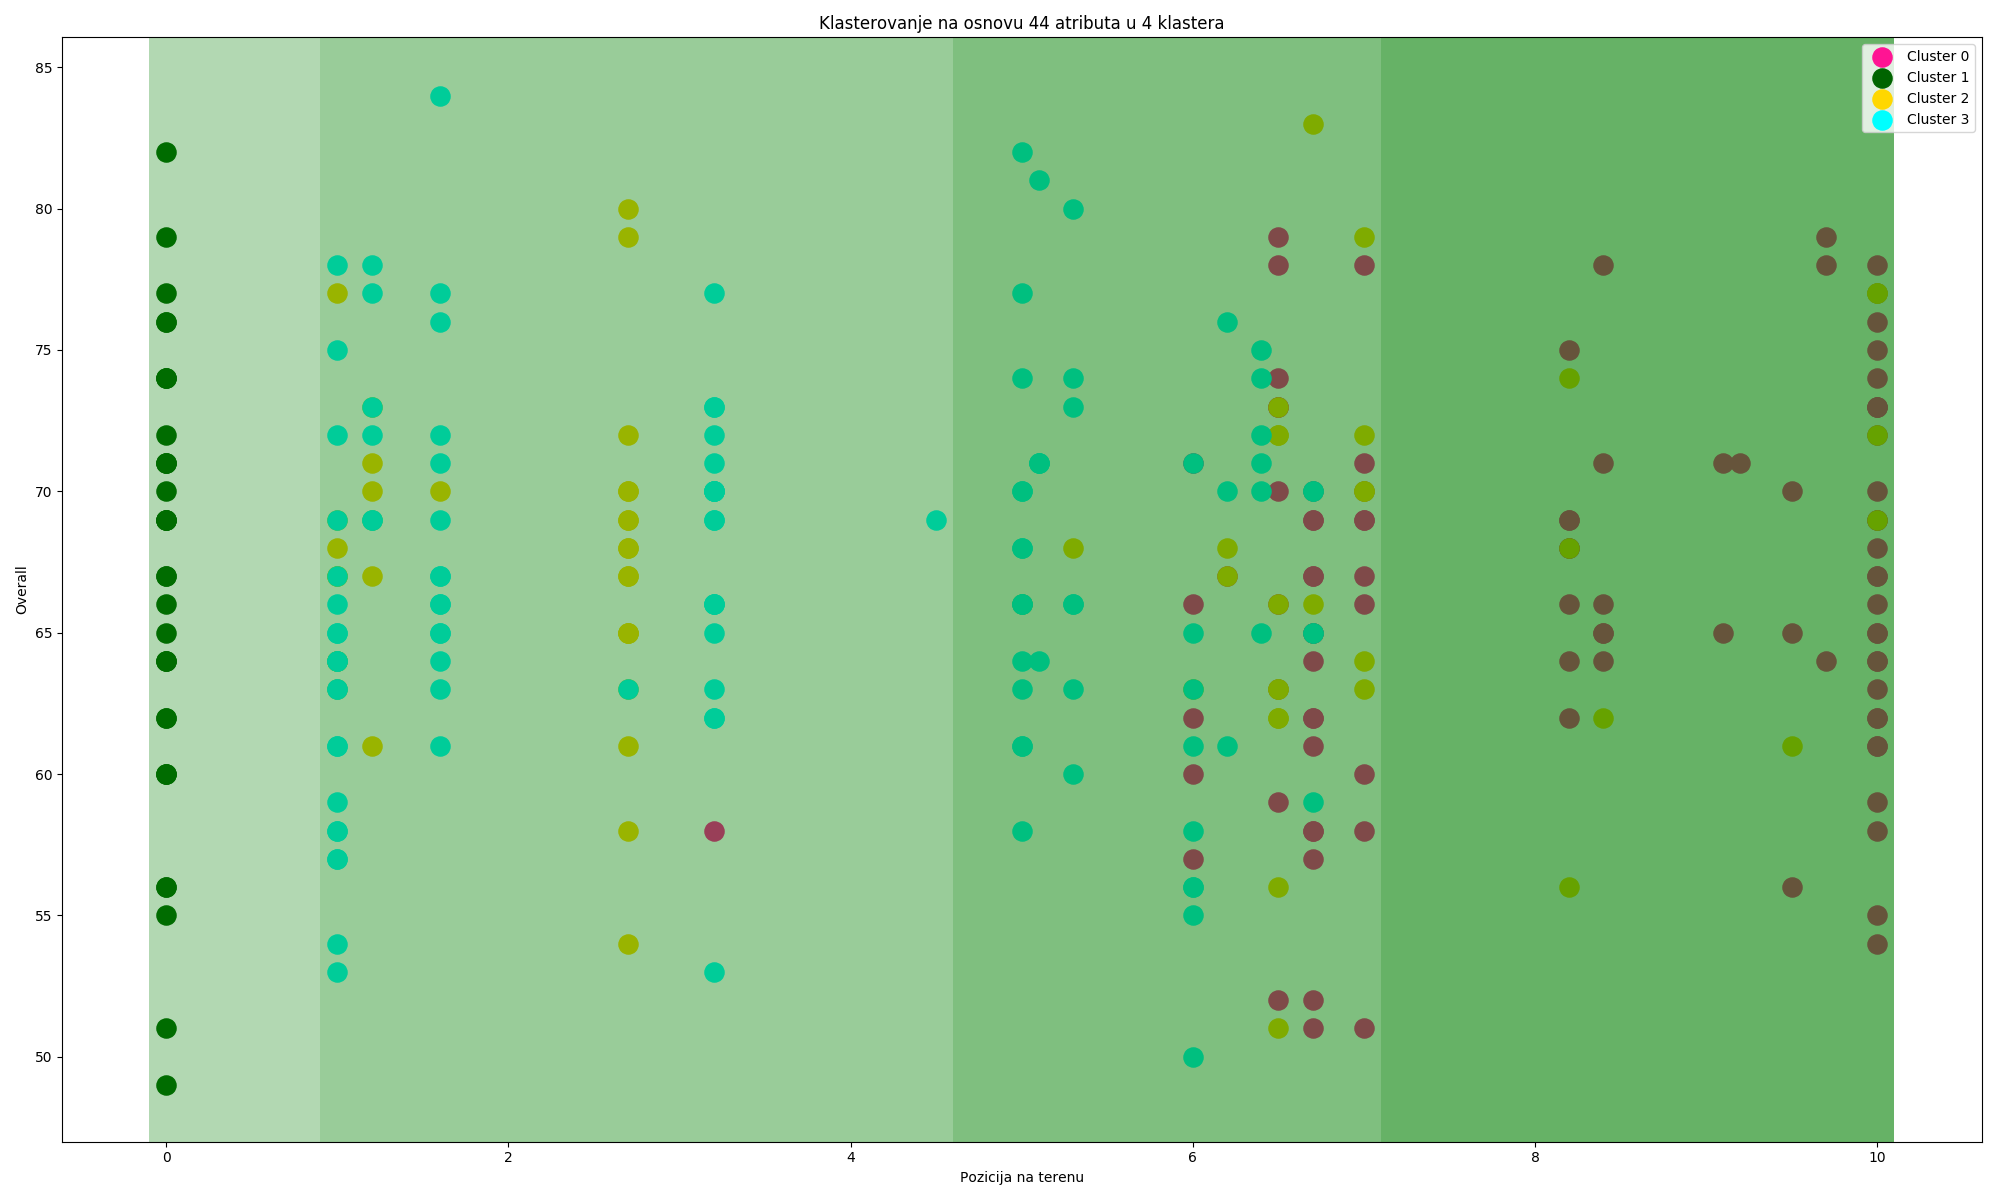
\includegraphics[scale=0.15]{position_clustering.png}
\caption{4-means Position $\sim$ Overall}
\end{figure}


Jasno se vidi da je klasterovanje relativno uspe\v{s}no, 
golmani su perfektno izdvojeni jer u skupu postoji 6 atributa 
karakteristi\v{c}nih za golmane. I oni prave jasnu distinkciju
izme\dj{}u golmana i igra\v{c}a u polju. U zajedni\v{c}ki
klaster su izdvojene i pozicije u napadu sa ofanzivnim veznim
pozicijama. Kao i pozicije \v{s}topera sa desnim bekovima i zadnjim veznim.
\v{S}to je opet o\v{c}ekivano jer posao zadnjih veznih i \v{s}topera je 
da "kvare"  igru protivnika pa su ti atributi izra\v{z}eniji, dok je za desne
bekove pomalo iznena\dj{}uju\'{c}e.\\

Po sli\v{c}noj intuiciji (11 igra\v{c}a na teren) isproban je algoritam za parametre
$k=11 $ ,$ tol=1e-5$

\begin{figure}[h]
\centering
\graphicspath{{../}}
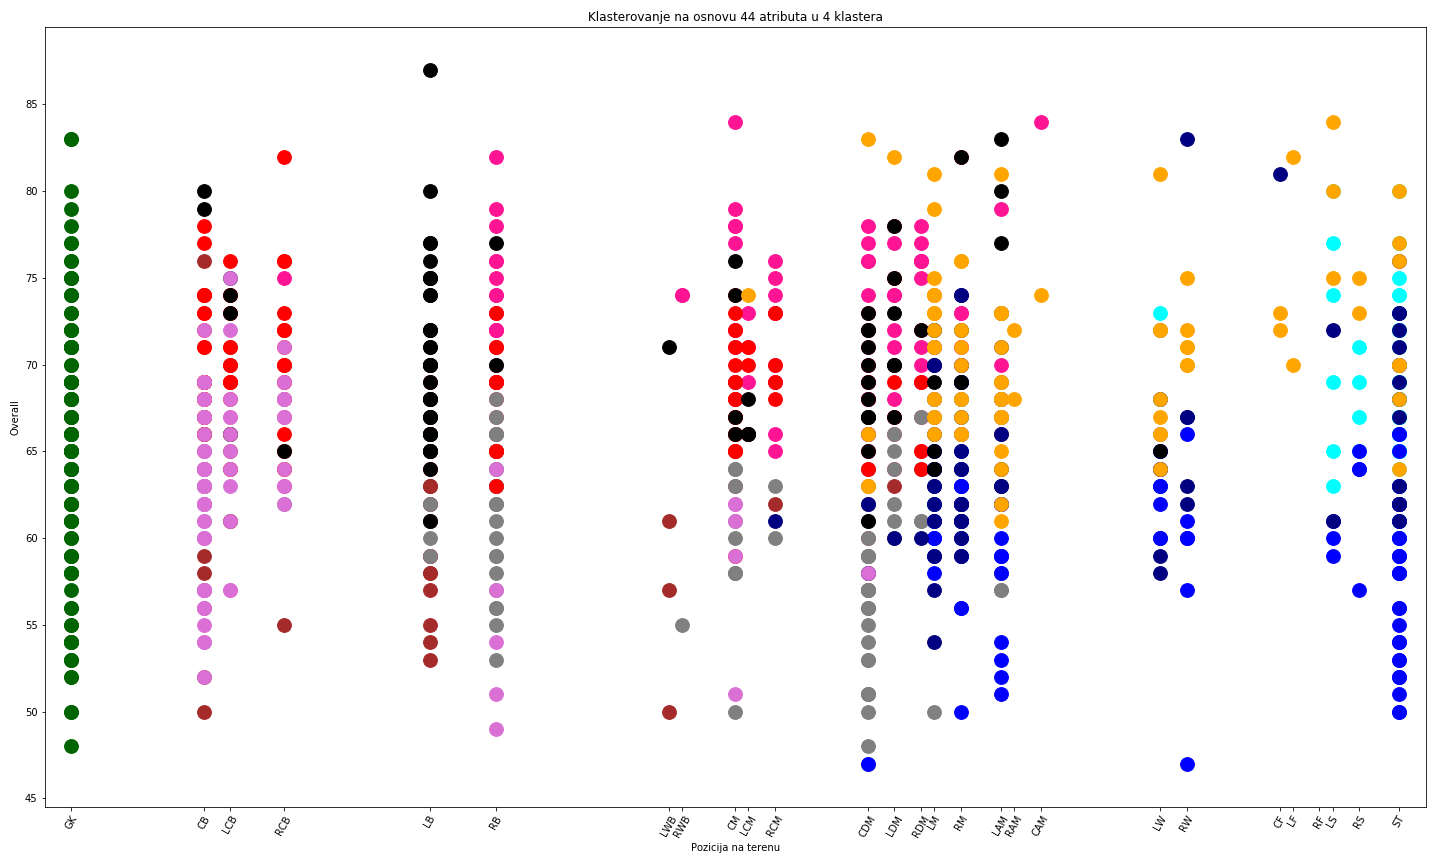
\includegraphics[scale=0.15]{kmeans_11.png}
\caption{11-means Position $\sim$ Overall}
\end{figure}

Sli\v{c}an rezultat\footnote{U oba slu\v{c}aja na grafiku je prikazan dosta manji slu\v{c}ajan
uzorak u odnosu na ceo skup podataka} je dobijen i ovde, tako da umesto dobijemo 11 klastera vezanih za svaku 
poziciju, dobili smo 4 ve\'{c}a klastera po pozicijama i posle podele tih klastera na manje
u odnosu na kvalitet igra\v{c}a na tim pozicijama.\\
\emph{Senka koeficijent} dobijen ovakvim klasterovanjem je 0.176189407.





\subsection{DBSCAN}
Ako bi samo primenili algoritam na ceo skup, sa ulaznim parametrima
$ \epsilon = 0.2 $ i MINSAMPLE=0.25 rezultati su katastrofalni.

\begin{figure}[h]
\centering
\graphicspath{{../}}
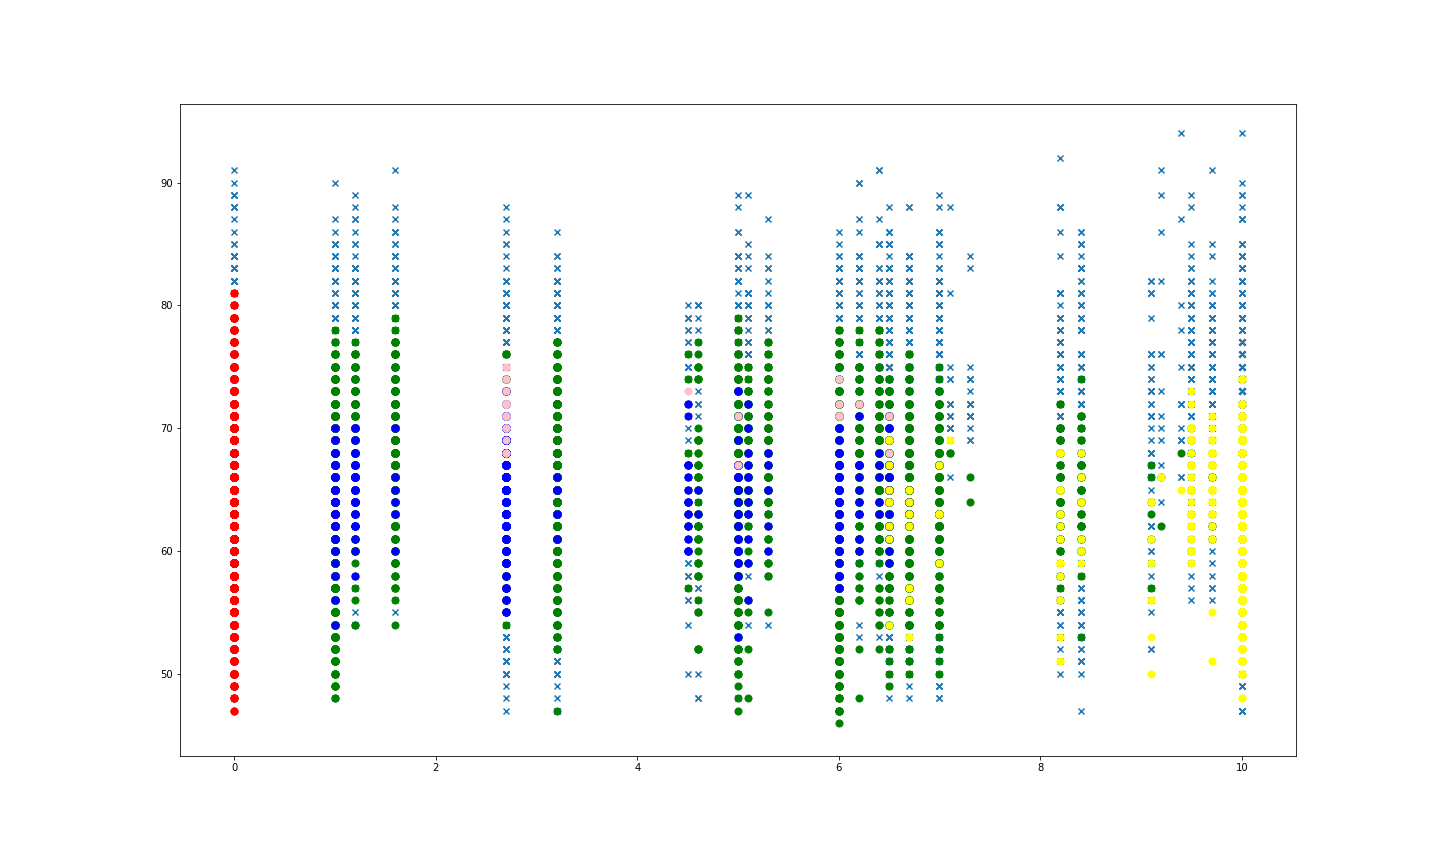
\includegraphics[scale=0.2]{dbscan_pca_020_25.png}
\caption{dbscan Position $\sim$ Overall}
\end{figure}



Ovaj algoritam je dao najlo\v{s}ije rezultate u radu sa celim skupom,
pa je uz pomo\'{c} algoritma PCA razbijen na 5 komponenata.
Pa je nad njima izvr\v{s}eno testirnje za kombinacije parametara.
I dobijeni su slede\'{c}i rezultati za \emph{senka koeficijent}:\\
{\scriptsize
EPS: 0.2, MINSAMPLE 15, -0.1869359996151717\\
EPS: 0.2, MINSAMPLE 17, -0.16759585821982464\\
EPS: 0.2, MINSAMPLE 19, -0.2173351910035472\\
EPS: 0.2, MINSAMPLE 22, -0.11936531330028984\\
EPS: 0.2, MINSAMPLE 25, -0.1105914961339661\\
EPS: 0.25, MINSAMPLE 15, 0.020336130534418833\\
EPS: 0.25, MINSAMPLE 17, -0.07882488012519194\\
EPS: 0.25, MINSAMPLE 19, -0.013699088736421575\\
EPS: 0.25, MINSAMPLE 22, 0.08744345584290553\\
EPS: 0.25, MINSAMPLE 25, -0.000881245667701518\\
EPS: 0.28, MINSAMPLE 15, 0.1888508085038652\\
EPS: 0.28, MINSAMPLE 17, 0.10032136758996933\\
EPS: 0.28, MINSAMPLE 19, 0.10049425982754563\\
EPS: 0.28, MINSAMPLE 22, 0.05128258301759307\\
EPS: 0.28, MINSAMPLE 25, 0.10400024000298268\\
EPS: 0.3, MINSAMPLE 15, 0.21026581196557972\\
EPS: 0.3, MINSAMPLE 17, 0.09208329293314058\\
EPS: 0.3, MINSAMPLE 19, 0.20001618066160468\\
EPS: 0.3, MINSAMPLE 22, 0.12226020063683611\\
EPS: 0.3, MINSAMPLE 25, 0.1196769498036405\\
\textbf{EPS: 0.35, MINSAMPLE 15, 0.2683946717146196}\\
EPS: 0.35, MINSAMPLE 17, 0.26255846338140093\\
EPS: 0.35, MINSAMPLE 19, 0.2588889497655407\\
EPS: 0.35, MINSAMPLE 22, 0.24745750354415014\\
EPS: 0.35, MINSAMPLE 25, 0.19363694433779471\\
\par}

Kada grafi\v{c}ki predstavimo klastere dobijene za najbolje ulazne parametre
vidimo da on jeste dobar ali da pravi samo 2 klastera. I to verovatno
samo na onu najve\'{c}u podelu golman-igra\v{c}i u polju. Pa nam i ne daje
neke zna\v{c}ajnije informacije.


\begin{figure}[h]
\centering
\graphicspath{{../}}
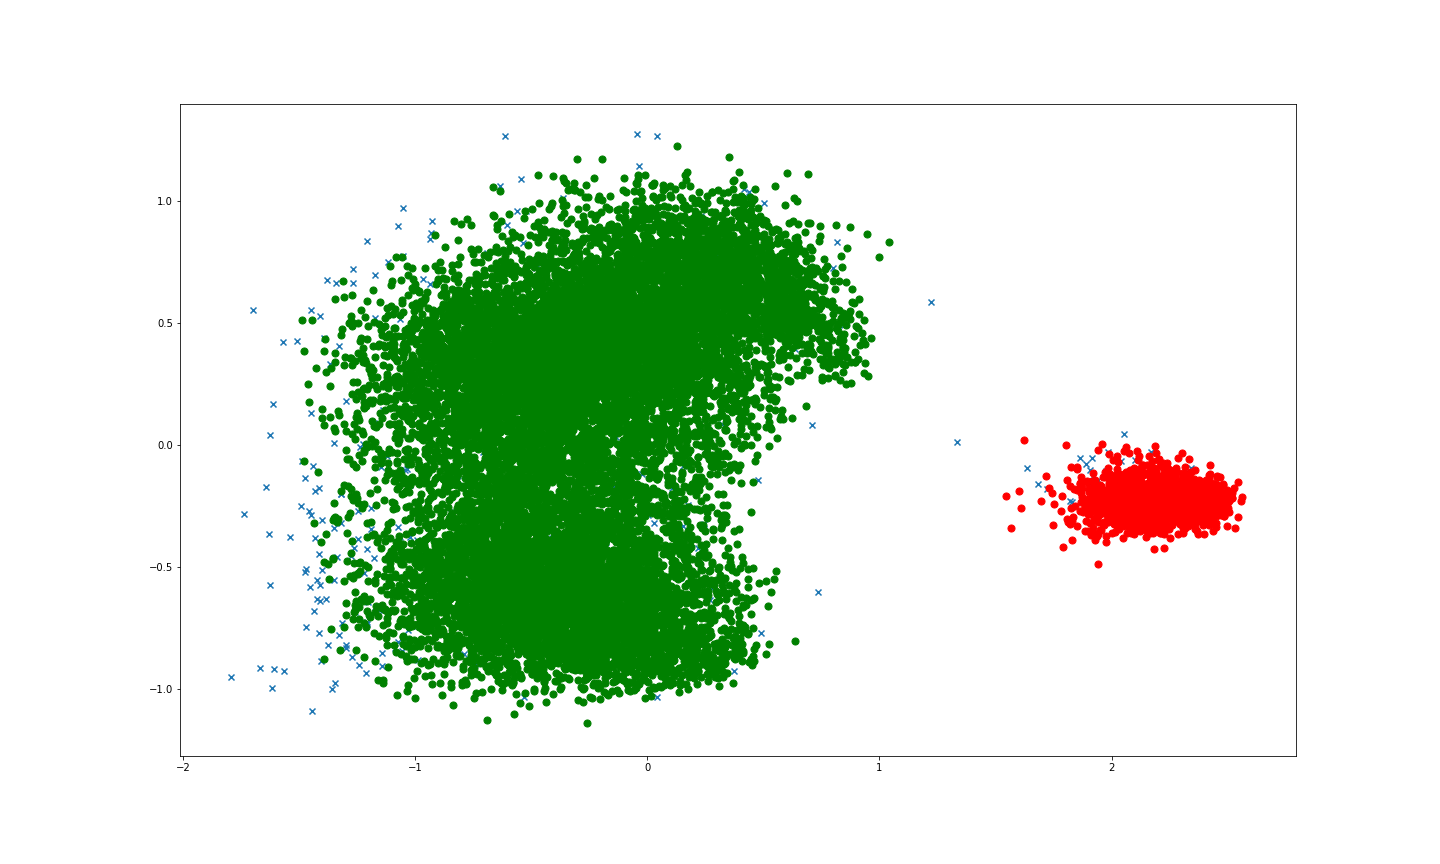
\includegraphics[scale=0.15]{dbscan_pca_035_15.png}
\caption{dbscan pca1 $\sim$ pca2}
\end{figure}


Jedan od razloga za ovakvo pona\v{s}anje ovog algoritma bi mogao da bude
taj \v{s}to vrednosti atributa nisu gusto raspore\dj{}ene po celom skupu.
Ve\'{c}ina ih se u po\v{c}etku nalazi u opsegu od 40 celobrojnih vrednosti.
Pa i kad se skaliraju nisu skroz gusto postavljeni na realnoj pravoj.
Zato je te\v{s}ko na\'{c}i razmeru $\epsilon$ i MINSAMPLE u cilju pove\'{c}anja
broja klastera, a ne naru\v{s}avanju njihovog kvaliteta. 

\subsection{Self Organizing Maps}

Algoritam Kohonen primenjen u spss na sve podatke daje rezultate:
\begin{figure}[h]
\centering
\graphicspath{{../}}
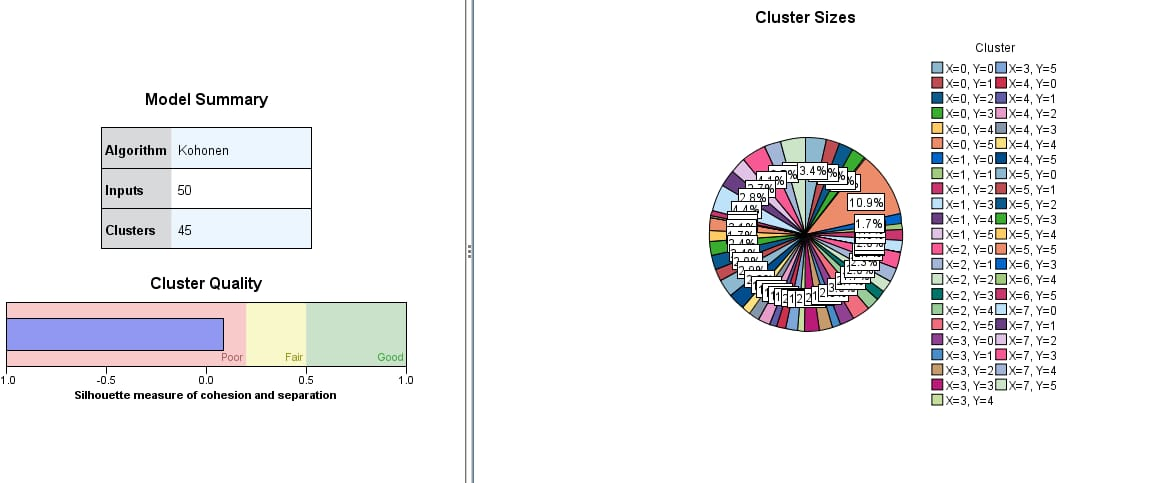
\includegraphics[scale=0.35]{kohonen_spss.jpeg}
\caption{SPSS Kohonen}
\end{figure}

Na \v{z}alost ovoliki broj klastera nam ne zna\v{c}i.
Va\v{z}nost atributa u svakom od klastera mogu\'{c}e je videti 
\href{www.alas.matf.bg.ac.rs/~mi16077/kohonen.jpeg}{ovde}.
\\

Poku\v{s}alo se i primenom istog algoritma uz pomo\'{c} PCA,
iz Python modula \emph{minisom} na mre\v{z}i 3x3.

\begin{figure}[h]
\centering
\graphicspath{{../}}
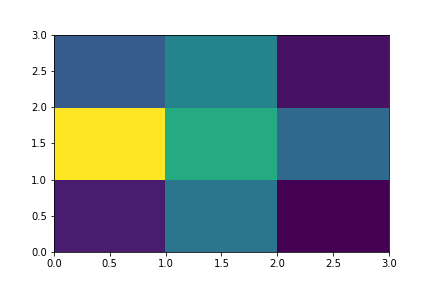
\includegraphics[scale=0.45]{distance_map_som.png}
\caption{Distance Map}
\end{figure}

\begin{figure}[h]
\centering
\graphicspath{{../}}
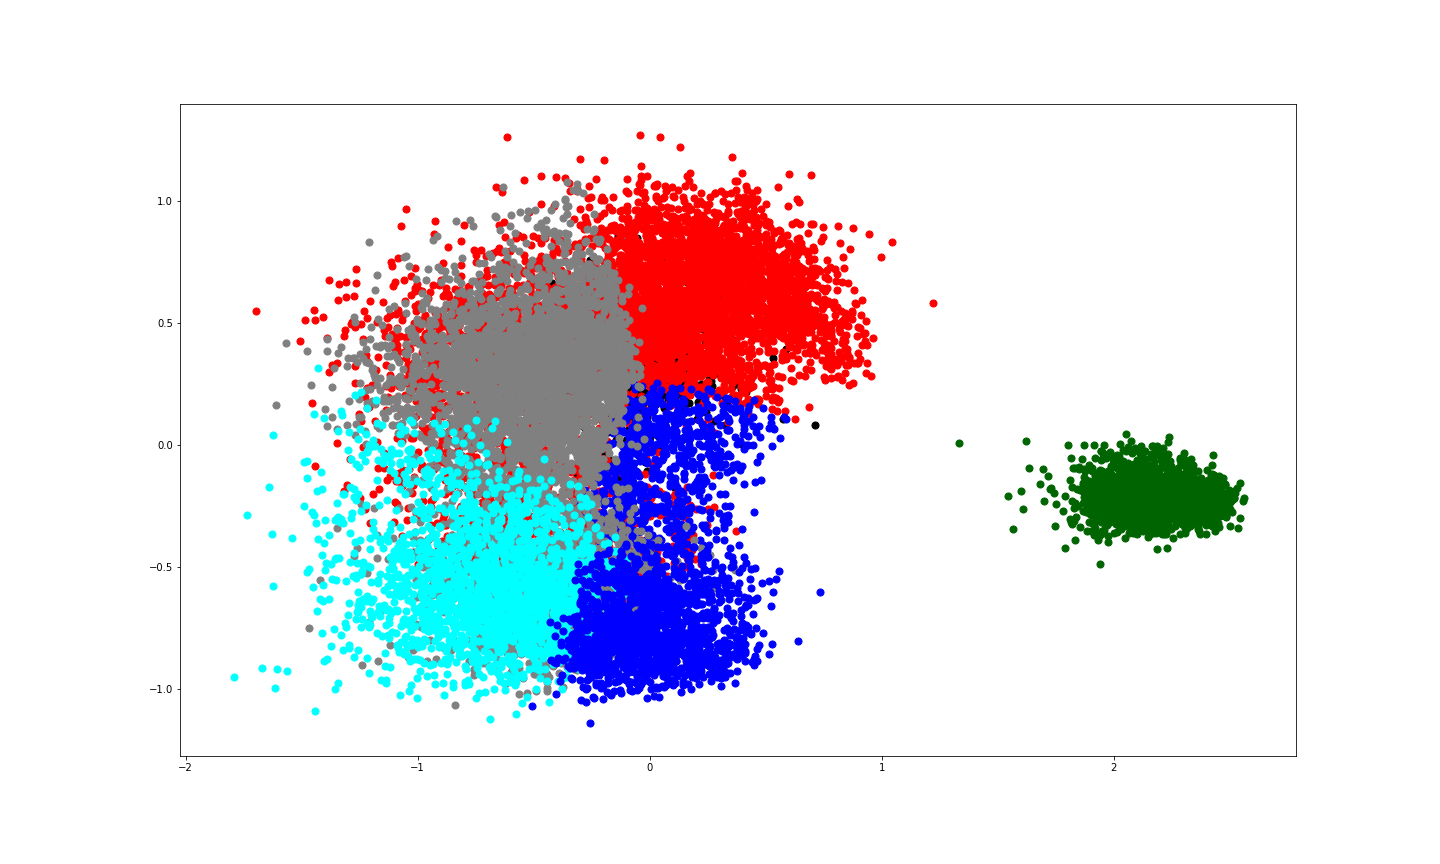
\includegraphics[scale=0.15]{som_pca5.png}
\caption{SOM pca}
\end{figure}


Vidimo da je \emph{senka koeficijent} sli\v{c}an onom 
dobijenom pomo\'{c}u softvera SPSS Modeler.
Tako da i ovaj poku\v{s}aj mo\v{z}emo podvesti pod
neuspe\v{s}an.



\subsection{Hijerahijsko klasterovanje}
Aglomerativni algoritam je odmah testiran za kombinacije ulaznih parametara.\\

{\scriptsize
\begin{multicols}{2}
complete
3:
0.16111395901587666\\

complete
4:
0.15463340908414164\\

complete
5:
0.10867388502724341\\

complete
6:
0.10899681823968788\\

complete
7:
0.1163346869599695\\

complete
8:
0.08395732844533542\\

complete
9:
0.07767909227419069\\

complete
10:
0.06966049001459615\\

average
3:
0.2709627878327729\\

average
4:
0.24091917722313702\\

average
5:
0.1728780322782311\\

average
6:
0.11372869517045374\\

average
7:
0.0960059077583922\\

average
8:
0.08104887570408535\\

average
9:
0.07844464901824208\\

average
10:
0.060803301819689466\\

single
3:
0.4411833673662859\\

single
4:
0.41806554059568624\\

single
5:
0.4043615186449922\\

single
6:
0.25612808527919223\\

single
7:
0.2544154870862858\\

single
8:
0.25318604389230687\\

single
9:
0.24743314095736932\\

single
10:
0.19687832678703504\\

ward
3:
0.24043039484247533\\

ward
4:
0.2380921126774734\\

ward
5:
0.1895722289010395\\

ward
6:
0.19807178307014062\\

ward
7:
0.16971785435757866\\

ward
8:
0.16611285555102587\\

ward
9:
0.15481562166653126\\

ward
10: 
0.15596833147946337
\end{multicols}
}
Nakon \v{s}to je prime\'{c}eno da single veza daje najbolje rezultate.
Primenjen je algoritam ponovo za broj klastera 11.

\begin{figure}[h]
\centering
\graphicspath{{../}}
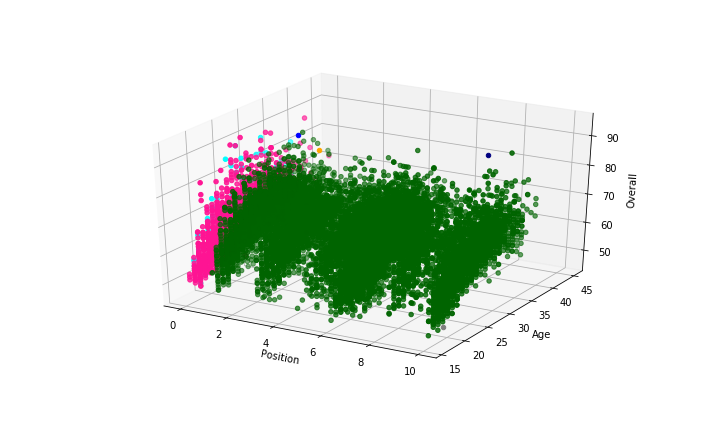
\includegraphics[scale=0.45]{agglomerative_11_3d_overall_age_position.png}
\caption{Agg11 Overall $\approx$ Age $\approx$ Position}
\end{figure}
O\v{c}igledno i ovog put razdvaja dva najve\'{c}a klastera, \v{c}ak
i me\dj{}u golmanima pronalazi potklastere. \\

Isprobano je sa istim parametrima primeniti algoritm i na podatke 
redukovane sa PCA:

\begin{figure}[h]
\centering
\graphicspath{{../}}
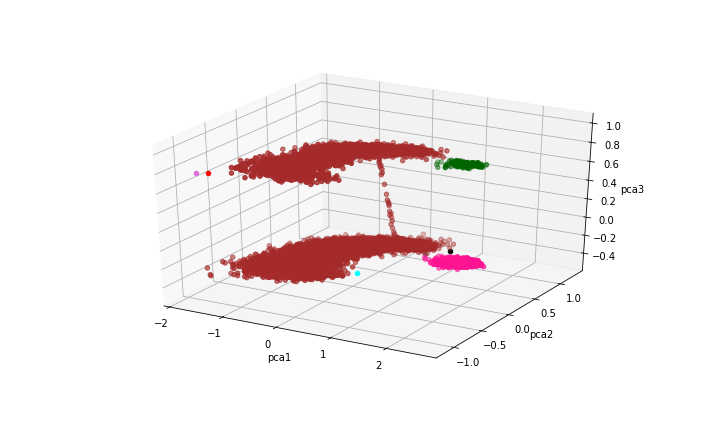
\includegraphics[scale=0.45]{agglomerative_11_pca_3d.png}
\caption{Agg11 PCA}

\end{figure}
Jedna zanimljivost, pri ovakvoj klasterizaciji pojavljuju se 3 klastera sa samo 
po jednim objektom. U kojima se nalaze redom : po mnogima najbolji fudbaler
svih vremena Lionel Messi, golman iz Japana od 42 godine i golman iz Indije
koji je trenutno bez kluba, kom zapravo u skupu podataka i nedostaje vrednost
za atribut pozicije na kojoj igra. Pa je pri interpolaciji svrstan u igra\v{c}e
u polju to jest vrednost \emph{Position} je $  >0$  

\subsection{Mean-shfit}
Mean-shift algoritam je jo\v{s} algoritam kod kog nije mogu\'{c}e kao parametar
zadati broj klastera koji \v{z}elimo da izdvojimo. Ve\'{c} zadajemo okolinu
(\emph{engl. bandwidth}). \\

\begin{lstlisting}[language=Pascal]
Input: bandwith, skup podataka
WHILE postoji objekat koji nije dodeljen nijednom klasteru DO:
		izaberi jedan od nedodeljenih objekata i označi
		da pripada novom klasteru
		REPEAT:
			azuriraj srednju tacku(centroid) u trenutnom klasteru;
			sve tačke koje se nalaze na razdaljini manjoj
			od bandwidth oznaci ih da pripadaju trenutnom
			klasteru
		UNTIL postoji promena na trenutnom klasteru
\end{lstlisting}

Paramtear bandwidth je u prvom testu izabran uz pomo\'{c}
\emph{sklearn.estimate\_bandwidth()}, rezultat klasterovanja
sa ovakvim izborom je odli\v{c}an \emph{senka koeficijent},
ali sa samo 2 klastera.
Pa je smanjen parametar sa 1.5 na 0.5, smanjen je \emph{senka
koeficijent}, ali je broj klastera bio 7.


\begin{figure}[h]
\centering
\graphicspath{{../}}
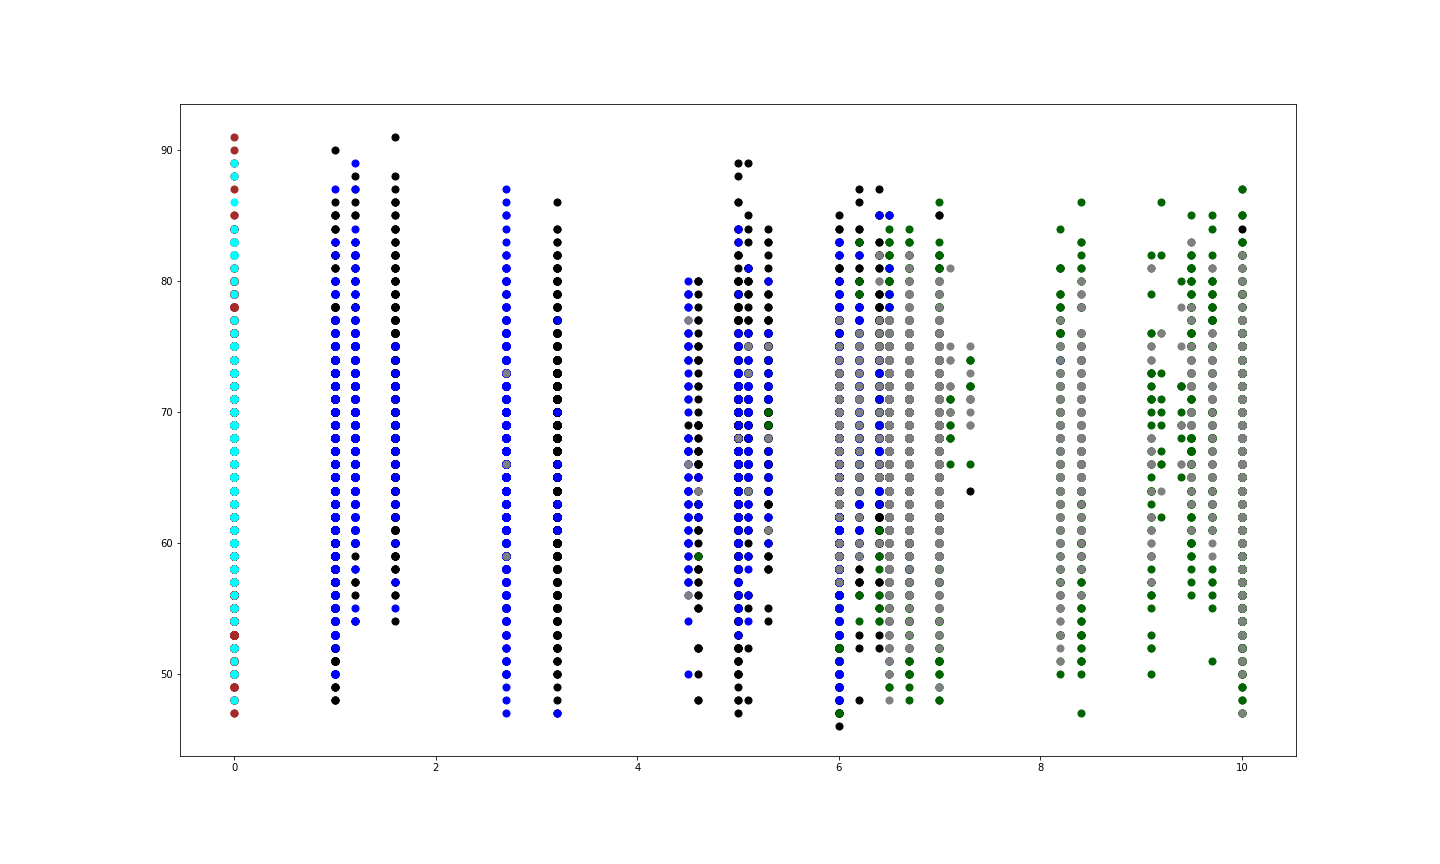
\includegraphics[scale=0.2]{meanshift_bandwith05.png}
\caption{Meanshift}
\end{figure}

\v{C}ak i sa ovim pogor\v{s}anjem \emph{senka koeficijenta}
on ostaje iznad vrednosit 0.5
Klastera ima vi\v{s}e nego pri 4-means algoritmu, ali 
manje su raspr\v{s}eni po terenu.

\begin{figure}[h]
\centering
\graphicspath{{../}}
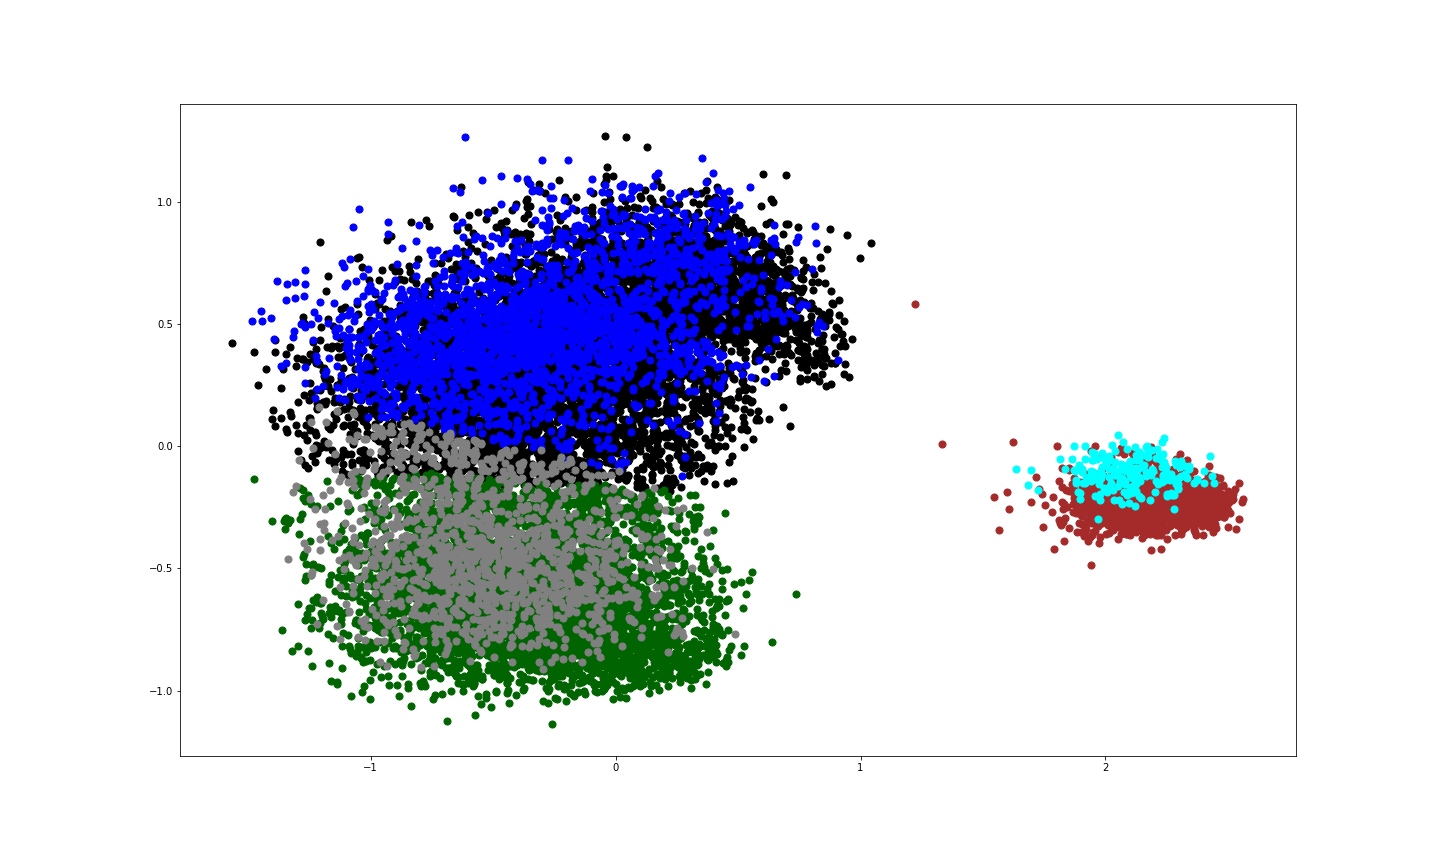
\includegraphics[scale=0.2]{meanshift_bandwith05_pca.png}
\caption{Meanshift PCA}
\end{figure}


\subsection{BIRCH}

BIRCH - \emph(balanced iterative reducing and clustering using hierarchies)
Hibridni algoritam za klasteorvanje koji se zasniva na pravljenju
CF(\emph{Clusters Features})-stabla. Kasnijim particionisanjem
stabla od korena ka vrhu stvaraju\'{c}i klastere.
\\
Za paramtera $k = 11$ Birch daje sli\v{c}ne rezultate kao i 11-means.


\begin{figure}[h]
\centering
\graphicspath{{../}}
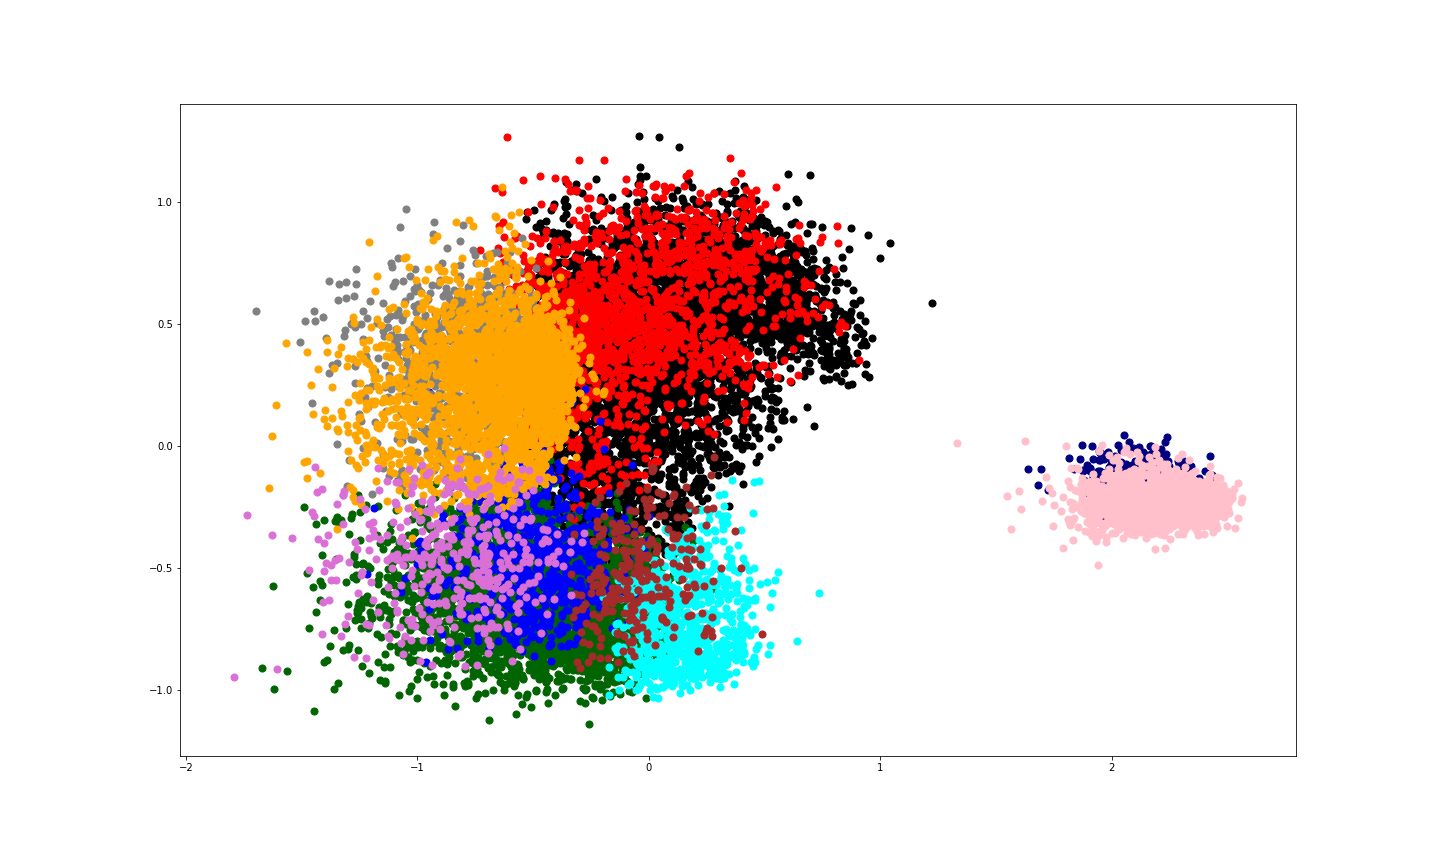
\includegraphics[scale=0.2]{birch_11_pca.png}
\caption{BIRCH PCA}
\end{figure}

Ali primenom na PCA komponente dobijamo \emph{senka koeficijent} $\approx 0.61$
sa 11 klastera. \v{S}to je definitivno najbolji pojedina\v{c}ni rezultat
dobijen tokom izrade ovog seminarskog rada.


\section{Zaklju\v{c}ak}
Skup podataka FIFA19 je verovatno jedan od popularnijih na
adresi: \url{www.kaggle.com}, \v{s}to zbog popularnosti tematike
tako i velikog broja atributa koje je mogu\'{c}e kombinovati i izvla\v{c}enja
finijih podela i filtriranja. U ovom seminarskom radu je nije bilo prostora uraditi
mnogo finijih klaster analiza na u\v{z}im podskupovima i sa drugim ciljevima.
Pa je izabran najintuitvniji cilj. Podela do 11 klastera nad svim igra\v{c}ima
i opet su napravljeni solidni rezultati.

Algoritmi DBSCAN i SOM su se pokazali lo\v{s}ije od ostalih,
dok ostala 4 algoritma je uz dodatno testiranje parametara
mogu\'{c}e podesiti da daju sli\v{c}ne rezultate. \\

Celokupan materijal kori\v{s}\'{c}en u ovom seminarskom 
radu \'{c}e do daljenjg biti dosptupan na adresi:
\url{https://github.com/gianthead97/fifa_19_clustering}.


\end{document}
